
\documentclass[tikz]{standalone}
\usepackage{tikz}
\usetikzlibrary{fit}
\usepackage[dvipsnames]{xcolor}
\usetikzlibrary{positioning, arrows.meta, calc, decorations.pathreplacing}
\definecolor{lightblue}{RGB}{173, 216, 230}
\begin{document}
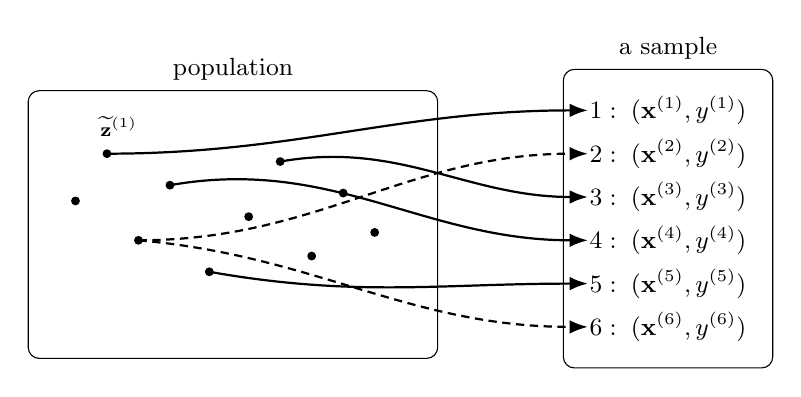
\begin{tikzpicture}[>=Latex, font=\small]
 \node[draw, rounded corners, inner sep=6pt,
 minimum width=5.2cm, minimum height=3.4cm] (pop) {};
 \node[above=0pt of pop.north] {population};
 \foreach \x/\y [count=\i] in {-2.0/0.3, -1.6/0.9, -1.2/-0.2, -0.8/0.5,
 -0.3/-0.6, 0.2/0.1, 0.6/0.8, 1.0/-0.4,
 1.4/0.4, 1.8/-0.1} {
 \coordinate (p\i) at ($(pop.center)+(\x,\y)$);
 \fill (p\i) circle (1.6pt);
 }
 \coordinate (sampleanchor) at ([xshift=1.8cm,yshift=0.5cm]pop.east);
 \def\rowgap{0.55cm}
 \def\ybase{0.95cm}
 \node[anchor=west] (s1) at ($(sampleanchor)+(0, \ybase - 0*\rowgap)$)
 {$1:\;({\bf x}^{(1)},y^{(1)})$};
 \node[anchor=west] (s2) at ($(sampleanchor)+(0, \ybase - 1*\rowgap)$)
 {$2:\;({\bf x}^{(2)},y^{(2)})$};
 \node[anchor=west] (s3) at ($(sampleanchor)+(0, \ybase - 2*\rowgap)$)
 {$3:\;({\bf x}^{(3)},y^{(3)})$};
 \node[anchor=west] (s4) at ($(sampleanchor)+(0, \ybase - 3*\rowgap)$)
 {$4:\;({\bf x}^{(4)},y^{(4)})$};
 \node[anchor=west] (s5) at ($(sampleanchor)+(0, \ybase - 4*\rowgap)$)
 {$5:\;({\bf x}^{(5)},y^{(5)})$};
 \node[anchor=west] (s6) at ($(sampleanchor)+(0, \ybase - 5*\rowgap)$)
 {$6:\;({\bf x}^{(6)},y^{(6)})$};
 \node[draw, rounded corners, inner sep=6pt, fit=(s1)(s6)] (seqbox) {};
 \node[above=0pt of seqbox.north]
 {a sample};
 \node[font=\scriptsize] at ($(p2)+(1.5mm,3.5mm)$) {$\widetilde{{\bf z}}^{(1)}$};
 \draw[->, thick] (p2) to[out=0, in=180] ($(s1.west)+(1mm,0mm)$);
 \draw[->, thick] (p7) to[out=10, in=180] ($(s3.west)+(1mm,0mm)$);
 \draw[->, thick] (p4) to[out=10, in=180] ($(s4.west)+(1mm,0mm)$);
 \draw[->, thick] (p5) to[out=-10, in=180] ($(s5.west)+(1mm,0mm)$);
 \draw[->, thick, densely dashed] (p3) to[out=0, in=180] ($(s2.west)+(1mm,0mm)$);
 \draw[->, thick, densely dashed] (p3) to[out=-5, in=180] ($(s6.west)+(1mm,0mm)$);
 \end{tikzpicture}
\end{document}
